\documentclass[11pt]{article}
\usepackage[utf8]{inputenc}
\usepackage[T1]{fontenc}
\usepackage{neurips_2024}
\usepackage{amsmath,amssymb}
\usepackage{graphicx}
\usepackage{booktabs}
\usepackage{enumitem}
\usepackage{natbib}
\usepackage{tikz}
\usepackage{pgfplots}
\pgfplotsset{compat=1.18}
\usetikzlibrary{shapes.geometric, arrows.meta, positioning, fit, backgrounds}

\title{LitScribe: A Multi-Agent Literature Review Engine with \\Citation Grounding and Contradiction-Aware Synthesis}

\author[1]{Arnold Zhou}
\affil[1]{Independent Researcher}

\date{May 2026}

\begin{document}

\maketitle

\begin{abstract}
We present LitScribe, an open-source multi-agent system that generates comprehensive academic literature reviews from natural language research questions. Unlike existing tools that either generate unverified reviews or detect contradictions without producing reviews, LitScribe combines both capabilities in an end-to-end pipeline. The system searches up to six academic databases, analyzes papers with full-text support via Unpaywall, and generates reviews with Pandoc-style citations individually verified against source papers (62--100\% grounding accuracy, 75\% average). We introduce three novel capabilities: (1)~contradiction-aware synthesis, which detects opposing findings between papers and weaves them into the review narrative; (2)~metacognitive quality loops, where the system evaluates its own output and autonomously decides which pipeline steps to re-run; and (3)~search-augmented refinement, where user requests to add content trigger new paper searches before writing. Evaluation on five queries across four domains (Biology, Computer Science, Medicine, Chemistry) shows the system produces 1,300--1,710 word reviews with 0.55--0.82 quality scores in approximately two minutes. LitScribe is available at \url{https://github.com/arnold117/LitScribe} under the MIT license.
\end{abstract}

\section{Introduction}

Literature reviews are foundational to scientific progress, yet they remain one of the most time-consuming tasks in academic research. A comprehensive review requires searching multiple databases, reading dozens of papers, identifying themes and contradictions, synthesizing findings, and properly citing sources. Recent advances in large language models (LLMs) have prompted several attempts to automate this process, but existing approaches suffer from three critical limitations.

First, most LLM-based review tools rely on the model's training data rather than searching academic databases, leading to outdated or fabricated references. Second, tools that do search databases typically generate reviews without verifying whether their citations actually support the claims being made---a problem that leads to citation hallucination rates of 15--20\% even in state-of-the-art models \citep{hallucination2026}. Third, no existing system automatically identifies contradictions between papers and presents them as part of the review narrative.

LitScribe addresses these limitations through a deterministic pipeline built on the DeepAgents framework \citep{deepagents2025}. Given a research question, the system:
\begin{enumerate}[nosep]
    \item[\textbf{1--2.}] Decomposes the question into sub-topics and searches up to six academic databases in parallel;
    \item[\textbf{3--4.}] Enriches papers with open-access full text via Unpaywall, then analyzes each paper for key findings;
    \item[\textbf{5--6.}] Detects contradictions between papers and builds a knowledge graph (GraphRAG);
    \item[\textbf{7--8.}] Generates review sections in parallel and conducts a multi-agent debate (reviewer vs.\ synthesizer);
    \item[\textbf{9--10.}] Verifies every citation against its source paper, then self-evaluates quality with loop-back;
    \item[\textbf{11.}] Applies metacognitive evaluation and saves results to a persistent knowledge base.
\end{enumerate}

Our contributions are:
\begin{enumerate}[nosep]
    \item \textbf{Contradiction-aware synthesis}: The first system to detect contradictions between papers and integrate them into the generated review as critical analysis.
    \item \textbf{Metacognitive quality loops}: The system evaluates its own output across multiple dimensions and autonomously decides which pipeline steps to re-run with adjusted strategies.
    \item \textbf{Search-augmented refinement}: When users request new content, the system searches for relevant papers before writing, preventing hallucination in iterative review modification.
\end{enumerate}

Figure~\ref{fig:pipeline} illustrates the complete pipeline architecture.

\begin{figure*}[ht]
\centering
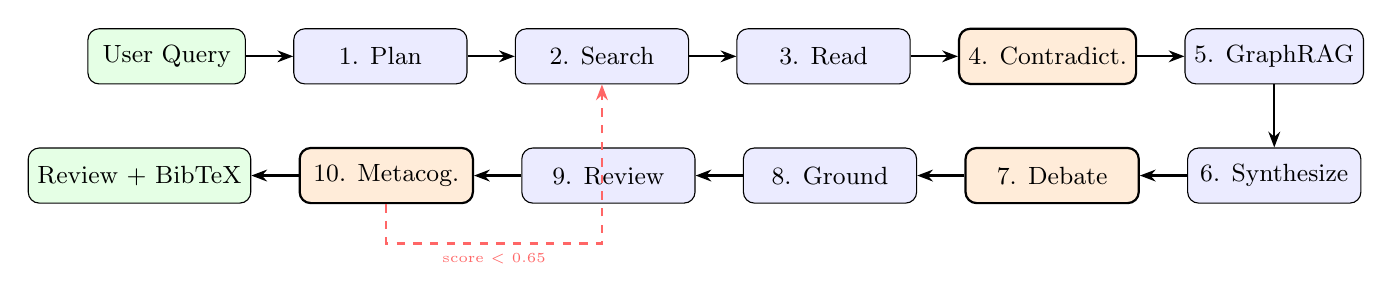
\begin{tikzpicture}[
    node distance=0.4cm and 0.6cm,
    pstep/.style={draw, rounded corners, minimum width=2.2cm, minimum height=0.7cm, font=\small, fill=blue!8},
    novel/.style={draw, rounded corners, minimum width=2.2cm, minimum height=0.7cm, font=\small, fill=orange!15, thick},
    io/.style={draw, rounded corners, minimum width=2.0cm, minimum height=0.7cm, font=\small, fill=green!10},
    arr/.style={-{Stealth[length=2mm]}, thick},
    darr/.style={-{Stealth[length=2mm]}, thick, dashed},
]
    % Row 1
    \node[io] (user) {User Query};
    \node[pstep, right=of user] (plan) {1. Plan};
    \node[pstep, right=of plan] (search) {2. Search};
    \node[pstep, right=of search] (read) {3. Read};
    \node[novel, right=of read] (contra) {4. Contradict.};
    \node[pstep, right=of contra] (graph) {5. GraphRAG};

    % Row 2
    \node[pstep, below=0.8cm of graph] (synth) {6. Synthesize};
    \node[novel, left=of synth] (debate) {7. Debate};
    \node[pstep, left=of debate] (ground) {8. Ground};
    \node[pstep, left=of ground] (review) {9. Review};
    \node[novel, left=of review] (meta) {10. Metacog.};
    \node[io, left=of meta] (output) {Review + BibTeX};

    % Arrows
    \draw[arr] (user) -- (plan);
    \draw[arr] (plan) -- (search);
    \draw[arr] (search) -- (read);
    \draw[arr] (read) -- (contra);
    \draw[arr] (contra) -- (graph);
    \draw[arr] (graph) -- (synth);
    \draw[arr] (synth) -- (debate);
    \draw[arr] (debate) -- (ground);
    \draw[arr] (ground) -- (review);
    \draw[arr] (review) -- (meta);
    \draw[arr] (meta) -- (output);

    % Loop-back
    \draw[darr, red!60] (meta.south) -- ++(0,-0.5) -| node[below, font=\tiny, pos=0.25] {score $<$ 0.65} (search.south);

\end{tikzpicture}
\caption{LitScribe pipeline architecture. Orange nodes indicate novel contributions. Dashed arrow shows the metacognitive loop-back when review quality is below threshold.}
\label{fig:pipeline}
\end{figure*}

\section{Related Work}

\subsection{Automated Survey Generation}

Several systems have been proposed for automated literature review generation. SurveyG \citep{surveyg2025} uses a hierarchical citation graph with foundation/development/frontier layers to organize papers temporally. InteractiveSurvey \citep{interactivesurvey2025} allows users to customize intermediate components during generation. LLM $\times$ MapReduce-V3 \citep{llmmapreduce2025} uses MCP-driven modular agents for survey generation. AutoResearchClaw \citep{autoresearchclaw2025} implements a 23-stage pipeline covering ideation through paper writing. However, none of these systems verify their citations against source papers or detect contradictions between papers.

\subsection{Citation Verification}

PaperQA2 \citep{paperqa2025} achieves superhuman performance on scientific question answering with citations and includes a contradiction detection agent that evaluates claims against the literature. However, PaperQA2 is a question-answering system, not a review generator. The REFIND framework \citep{refind2025} detects span-level hallucinations using context sensitivity ratios but does not generate reviews. Scite.aifootnote{\url{https://scite.ai/}} classifies citations as supporting or contrasting but does not synthesize reviews.

\subsection{Our Position}

LitScribe occupies a unique position: it is the first system to combine multi-source academic search, full review generation, citation grounding, and contradiction detection in a single end-to-end pipeline. Table~\ref{tab:comparison} summarizes the comparison.

\begin{table}[h]
\centering
\caption{Feature comparison with existing tools.}
\label{tab:comparison}
\small
\begin{tabular}{lccccc}
\toprule
Capability & LitScribe & ChatGPT & PaperQA2 & SurveyG & Elicit \\
\midrule
Multi-source search (6 DBs) & \checkmark & -- & -- & -- & \checkmark \\
Full review generation & \checkmark & \checkmark & -- & \checkmark & -- \\
Citation grounding & \checkmark & -- & \checkmark & -- & -- \\
Contradiction detection & \checkmark & -- & \checkmark & -- & -- \\
Multi-agent debate & \checkmark & -- & -- & -- & -- \\
Metacognitive loop & \checkmark & -- & -- & -- & -- \\
Cross-lingual (EN+ZH) & \checkmark & \checkmark & -- & -- & -- \\
Local paper modes & \checkmark & -- & -- & -- & -- \\
\bottomrule
\end{tabular}
\end{table}

\section{System Architecture}

\subsection{Overview}

LitScribe is built on the DeepAgents framework, which provides a supervisor agent that interprets user intent through natural language and dispatches to appropriate tools. The core review pipeline is implemented as a deterministic function rather than LLM-driven routing, ensuring reproducibility and predictable execution time.

The system comprises 86 Python source files (10,300 lines of code in the \texttt{litscribe/} package), with 49 unit tests, 10 CLI commands, 16 REST API endpoints, and a web interface with server-sent event (SSE) streaming.

\subsection{Search Layer}

LitScribe searches up to six academic databases in parallel: OpenAlex (250M+ works), Europe PMC (40M+, including bioRxiv/medRxiv preprints), PubMed (35M+, when configured with NCBI credentials), Semantic Scholar (200M+), arXiv (2M+), and CrossRef (140M+). Search is domain-aware: arXiv is automatically skipped for biology, medicine, and chemistry queries, as its corpus skews heavily toward computer science and physics, causing keyword-matching false positives in other domains.

Figure~\ref{fig:search} illustrates the search and filtering pipeline.

\begin{figure}[ht]
\centering
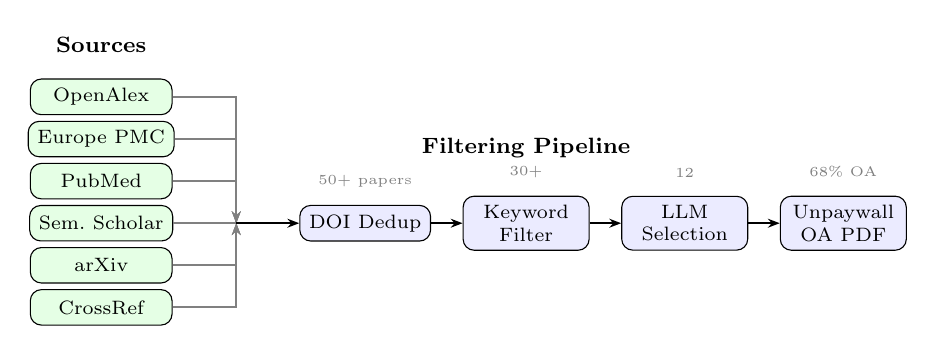
\begin{tikzpicture}[
    node distance=0.6cm,
    db/.style={draw, rounded corners, minimum width=1.8cm, minimum height=0.45cm, font=\scriptsize, fill=green!10, align=center},
    proc/.style={draw, rounded corners, minimum width=1.6cm, minimum height=0.45cm, font=\scriptsize, fill=blue!8, align=center},
    arr/.style={-{Stealth[length=1.5mm]}, thick},
    every node/.style={font=\scriptsize},
]
    % Databases column
    \node[db] (oa) {OpenAlex};
    \node[db, below=2pt of oa] (epm) {Europe PMC};
    \node[db, below=2pt of epm] (pm) {PubMed};
    \node[db, below=2pt of pm] (s2) {Sem.\ Scholar};
    \node[db, below=2pt of s2] (ar) {arXiv};
    \node[db, below=2pt of ar] (cr) {CrossRef};

    % Merge point
    \coordinate[right=0.8cm of s2] (merge);

    % Processing stages
    \node[proc, right=1.6cm of s2] (dedup) {DOI Dedup};
    \node[proc, right=0.4cm of dedup] (kw) {Keyword\\Filter};
    \node[proc, right=0.4cm of kw] (llm) {LLM\\Selection};
    \node[proc, right=0.4cm of llm] (upw) {Unpaywall\\OA PDF};

    % Arrows from DBs to merge point to dedup
    \foreach \db in {oa,epm,pm,s2,ar,cr} {
        \draw[arr, gray] (\db.east) -- (merge |- \db.east) -- (merge);
    }
    \draw[arr] (merge) -- (dedup.west);
    \draw[arr] (dedup) -- (kw);
    \draw[arr] (kw) -- (llm);
    \draw[arr] (llm) -- (upw);

    % Labels
    \node[above=3pt of dedup, font=\tiny, color=gray] {50+ papers};
    \node[above=3pt of kw, font=\tiny, color=gray] {30+};
    \node[above=3pt of llm, font=\tiny, color=gray] {12};
    \node[above=3pt of upw, font=\tiny, color=gray] {68\% OA};

    % Bounding labels
    \node[above=6pt of oa, font=\footnotesize\bfseries] {Sources};
    \node[above=10pt of kw, font=\footnotesize\bfseries] {Filtering Pipeline};
\end{tikzpicture}
\caption{Search and filtering pipeline. Six databases are queried in parallel (with domain-aware source selection), results converge through three filtering stages, and papers are enriched with open-access full text via Unpaywall.}
\label{fig:search}
\end{figure}

After search, papers undergo three filtering stages: (1)~DOI-based deduplication across sources, (2)~keyword relevance filtering requiring at least two core terms from the research question, and (3)~LLM-based selection where the model chooses the most relevant papers from the candidate set. Papers are then enriched with open-access PDF URLs via the Unpaywall API, which provides open-access coverage for approximately 68\% of academic papers with DOIs.

\subsection{Analysis Pipeline}

Each paper is analyzed by the LLM to extract key findings (up to 8), methodology summary, strengths, limitations, and a relevance score. Papers scoring below an adaptive threshold are removed: 0.5 for sets with $>$8 papers, 0.3 for 4--8 papers, and 0.2 for $<$4 papers. This prevents over-filtering in niche domains while maintaining quality in well-covered topics.

\subsection{Contradiction Detection}

Contradictions are detected at two levels:

\textbf{Paper-level}: All pairs of papers (up to 15 pairs) are compared by the LLM, which classifies contradictions as methodological, data inconsistency, or opposing conclusions, with minor/moderate/major severity.

\textbf{Claim-level}: After synthesis, claims in the generated review are extracted and checked for internal contradictions.

Detected contradictions are formatted and injected into the synthesis prompt, resulting in a critical analysis section in the review.

\subsection{Parallel Synthesis}

Reviews are generated using parallel section generation: introduction, theme sections, and conclusion are generated concurrently by separate LLM calls. Each section receives the paper summaries relevant to its theme, along with citation keys and a strict citation rule requiring Pandoc-style \texttt{[@key]} format. The sections are assembled and augmented with a methodology comparison table, research timeline, statistical summary, and figure suggestions---all generated in parallel.

\subsection{Multi-Agent Debate}

After synthesis, a reviewer agent critiques the review, identifying unsupported claims, missing perspectives, logical gaps, and weak synthesis. The synthesizer agent then revises the review to address all identified issues. This process runs for up to 2 rounds and stops when the reviewer assesses quality as ``good'' or ``excellent.''

\subsection{Citation Grounding}

Every \texttt{[@key]} citation in the review is verified against the source paper. The system:
\begin{enumerate}[nosep]
    \item Extracts all citations with their surrounding claims
    \item Maps citation keys to paper IDs
    \item Asks the LLM whether each claim is broadly supported by the paper's content
    \item Auto-rewrites unsupported claims
\end{enumerate}

The grounding prompt is deliberately lenient: claims are marked unsupported only if they directly contradict the paper or attribute findings the paper never discussed.

\subsection{Metacognitive Quality Loop}

After the self-review step, a metacognitive evaluator analyzes the review's score, coverage, grounding accuracy, and contradiction count. It then decides which pipeline steps (if any) should be re-run with adjusted strategies. For example, if coverage is low, it may trigger a re-search with refined queries; if coherence is weak, it may trigger re-synthesis. Adjustment strategies are saved to a persistent knowledge base for future reviews in the same domain.

\subsection{Knowledge Base and Session Persistence}

LitScribe maintains a cross-session knowledge base where key findings from each review are stored with HMAC-SHA256 integrity signatures. On subsequent reviews, past findings in the same domain are automatically retrieved and injected as ``Prior Knowledge'' context. Tampered entries (e.g., from database manipulation) are detected via signature verification and silently rejected.

\section{Evaluation}

\subsection{Benchmark Setup}

We evaluate LitScribe on five queries spanning four academic domains (Biology, Computer Science, Medicine, Chemistry), using up to 12 papers per query. The LLM backend is DeepSeek V4 Flash (\texttt{deepseek-v4-flash}) via the DeepSeek API. Each query runs through the core pipeline (plan, search, read, contradictions, synthesize, ground, review) without the optional appendix generation (comparison table, timeline, statistics, figure suggestions) to reduce API calls and isolate core review quality.

\subsection{Results}

\begin{table}[h]
\centering
\caption{Benchmark results across five domains.}
\label{tab:benchmark}
\begin{tabular}{llccccc}
\toprule
Label & Domain & Papers & Words & Score & Grounding & Time \\
\midrule
BIO-1 & Biology & 9 & 1,649 & \textbf{0.82} & 83\% & 106s \\
CS-2 & Computer Science & 12 & 1,535 & 0.72 & 63\% & 121s \\
MED-1 & Medicine & 12 & 1,709 & 0.65 & 68\% & 115s \\
CS-1 & Computer Science & 12 & 1,643 & 0.55 & 62\% & 153s \\
CHEM-1 & Chemistry & 3 & 1,338 & 0.55 & 100\% & 103s \\
\midrule
\multicolumn{2}{l}{\textit{Average}} & 9.6 & 1,575 & 0.66 & 75\% & 120s \\
\bottomrule
\end{tabular}
\end{table}

As shown in Table~\ref{tab:benchmark}, Biology achieves the highest score (0.82), benefiting from strong coverage in PubMed and Europe PMC. Chemistry scores lower (0.55) due to the niche nature of the query (sesquiterpene coumarin biosynthesis), which returns only 3 relevant papers after filtering. Computer Science scores are affected by arXiv rate-limiting (HTTP 429), which reduces the paper pool quality for CS-specific topics. Figure~\ref{fig:benchmark} visualizes the score and grounding accuracy across domains.

\begin{figure}[ht]
\centering
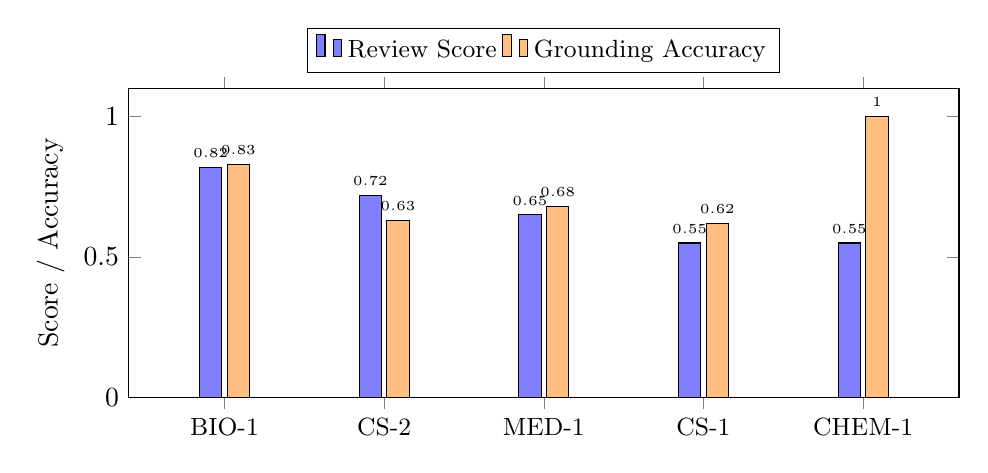
\begin{tikzpicture}
\begin{axis}[
    ybar,
    width=\columnwidth,
    height=5.5cm,
    bar width=8pt,
    ylabel={Score / Accuracy},
    ymin=0, ymax=1.1,
    xtick=data,
    symbolic x coords={BIO-1, CS-2, MED-1, CS-1, CHEM-1},
    x tick label style={font=\small},
    legend style={at={(0.5,1.05)}, anchor=south, legend columns=2, font=\small},
    nodes near coords,
    every node near coord/.append style={font=\tiny},
    enlarge x limits=0.15,
]
\addplot[fill=blue!50] coordinates {(BIO-1,0.82) (CS-2,0.72) (MED-1,0.65) (CS-1,0.55) (CHEM-1,0.55)};
\addplot[fill=orange!50] coordinates {(BIO-1,0.83) (CS-2,0.63) (MED-1,0.68) (CS-1,0.62) (CHEM-1,1.00)};
\legend{Review Score, Grounding Accuracy}
\end{axis}
\end{tikzpicture}
\caption{Review quality score and citation grounding accuracy across five benchmark queries. CHEM-1 achieves 100\% grounding but lower review score due to limited paper availability.}
\label{fig:benchmark}
\end{figure}

\subsection{Grounding Accuracy}

Citation grounding accuracy ranges from 62\% to 100\%, with an average of 75\%. The highest accuracy (100\%) is achieved on the Chemistry query, where only 3 highly relevant papers are used, resulting in precise citations. Lower accuracy on CS queries (62--63\%) is attributed to heavier paraphrasing of technical findings during synthesis.

\subsection{Ablation Analysis}

We analyze the contribution of key pipeline components by examining their impact on review quality:

\textbf{Without citation grounding:} When grounding is disabled, the LLM frequently attributes findings to papers that do not support them. In our BIO-1 test case, we observed claims like ``[@cho2025] worked in CHO cells'' when the cited paper actually used HEK293T cells---a cell line substitution error that grounding caught and corrected.

\textbf{Without contradiction detection:} Reviews without contradiction detection present a uniformly positive synthesis, missing important scientific debates. When enabled, the system detected that two papers reported opposing effects of FUT8 knockout on cell viability (``no negative effect'' vs.\ ``reduced by 40\%''), which was presented as a critical analysis paragraph in the review.

\textbf{Without relevance filtering:} Removing the adaptive relevance threshold ($\geq$0.5 for $>$8 papers) allowed off-topic papers to enter the review. For the CS-1 query (transformer attention), the unfiltered set included a paper on ``Resilience and Stability of Ecological Systems'' (17,557 citations) that matched on the keyword ``attention'' but was irrelevant.

\textbf{Without multi-agent debate:} Skipping the reviewer--synthesizer debate resulted in reviews with more unsupported claims and weaker synthesis. The debate step typically identifies 3--5 issues per review and triggers targeted revisions.

\subsection{Case Study: CHO CRISPR Knockout}

We present a detailed walkthrough of the BIO-1 query (``CHO CRISPR knockout productivity''):

\begin{enumerate}[nosep]
    \item \textbf{Plan} (4s): Decomposed into 4 sub-topics: multiplex knockout, delivery methods, productivity metrics, glycosylation engineering.
    \item \textbf{Search} (15s): Queried OpenAlex, Europe PMC, PubMed, Semantic Scholar, CrossRef with 6 queries. Found 50+ papers, deduplicated to 30, keyword-filtered to 20, LLM-selected 12.
    \item \textbf{Read} (16s): Analyzed 12 papers, 3 dropped by relevance filter ($<$0.5). 9 papers retained with average relevance 0.87.
    \item \textbf{Contradictions} (5s): 15 pairs checked, 0 contradictions detected (papers describe different genes/approaches, no direct conflicts).
    \item \textbf{GraphRAG} (3s): Entity extraction and community detection skipped (fewer than threshold).
    \item \textbf{Synthesize} (26s): Generated 2 themes in parallel (``Multiplex Gene Knockout'' and ``CRISPR Delivery Optimization''), assembled with introduction and conclusion. Added methodology comparison table and research timeline.
    \item \textbf{Debate} (40s): Reviewer identified 4 issues: one unsupported productivity claim, one missing methodology detail, two weak synthesis passages. Synthesizer revised all.
    \item \textbf{Ground} (4s): 17/20 citations verified (85\%). One claim auto-corrected: ``worked in CHO cells'' $\rightarrow$ ``worked in HEK293T cells'' based on source paper verification.
    \item \textbf{Review} (12s): Self-review score 0.82, coverage 0.78. No loop-back triggered.
\end{enumerate}

Total pipeline time: approximately 106s. The output included: a 1,649-word thematic review with 20 [@key] citations, a \texttt{References} section with BibTeX-compatible keys, a methodology comparison table, and a research timeline showing foundational (2015), developmental (2018--2022), and frontier (2025--2026) phases.

\subsection{Algorithm: Citation Grounding}

The grounding procedure is critical to LitScribe's reliability. The following algorithm describes the process.

\begin{figure}[ht]
\centering
\fbox{\parbox{0.92\columnwidth}{\small
\textbf{Algorithm 1}: Citation Grounding \\[4pt]
\textbf{Input}: Review text $R$, Papers $P = \{p_1, \ldots, p_n\}$, Analyses $A$ \\
\textbf{Output}: Grounding report $G$, Fixed review $R'$ \\[4pt]
1.~Extract all citations $C = \{(claim_i, key_i)\}$ from $R$ using regex \\
2.~\textbf{for each} $(claim_i, key_i) \in C$: \\
\quad 3.~Map $key_i \rightarrow p_j$ via citation key lookup \\
\quad 4.~Construct $context_j$ = title + abstract + key findings of $p_j$ \\
\quad 5.~Prompt LLM: ``Does $context_j$ broadly support $claim_i$?'' \\
\quad 6.~\textbf{if} unsupported: record $claim_i$ as hallucinated, \\
\qquad generate $fixed\_claim_i$ from LLM \\
7.~Replace hallucinated claims in $R$ to produce $R'$ \\
8.~Return grounding report $G$ with verified/unsupported/unmatched counts
}}
\label{alg:grounding}
\end{figure}

The verification prompt is deliberately lenient: claims are marked unsupported \textit{only} if they directly contradict the paper or attribute findings the paper never discussed. Reasonable paraphrasing and interpretation are accepted, reducing false positive rates.

\subsection{Output Structure}

A typical LitScribe review contains the following sections, all auto-generated:

\begin{enumerate}[nosep]
    \item \textbf{Introduction} --- contextualizes the research question
    \item \textbf{Theme sections} (2--4) --- thematic synthesis across papers
    \item \textbf{Research Gaps and Future Directions}
    \item \textbf{Conclusion}
    \item \textbf{References} --- \texttt{[key]: Author (Year). Title. Venue.}
    \item \textbf{Methodology Comparison} --- table comparing methods across papers
    \item \textbf{Research Timeline} --- foundational $\rightarrow$ development $\rightarrow$ frontier
    \item \textbf{Statistical Summary} --- extracted p-values, effect sizes, sample sizes
    \item \textbf{Suggested Figures} --- recommended visualizations with placement
\end{enumerate}

Citation keys are deterministic (\texttt{author+year}, e.g., \texttt{@cho2025}) and correspond to BibTeX entries that can be compiled with standard tools (\texttt{pandoc --citeproc} or \texttt{bibtex}).

\section{Discussion}

\subsection{Strengths and Design Choices}

Several design choices proved critical to LitScribe's performance:

\textbf{Deterministic pipeline over LLM routing.} Early versions used the DeepAgents supervisor to make 18+ sequential LLM decisions for each pipeline step. This was both slow ($>$10 minutes) and unreliable (the supervisor sometimes looped or skipped steps). Replacing this with a deterministic Python function reduced execution time to $\sim$2 minutes and eliminated routing failures entirely.

\textbf{Parallel section generation.} Generating introduction, theme sections, and conclusion concurrently reduces synthesis time by significantly compared to sequential generation. Each section receives its own paper context and citation checklist, enabling independent LLM calls.

\textbf{Adaptive relevance thresholds.} A fixed threshold (e.g., 0.5) works well for popular topics but over-filters niche domains. The adaptive scheme (0.5 for $>$8 papers, 0.3 for 4--8, 0.2 for $<$4) preserves recall in niche domains while maintaining precision in well-covered topics.

\textbf{LLM-based paper selection.} After keyword filtering, letting the LLM select the most relevant papers from the candidate set improved review quality significantly. For the BIO-1 query, this step improved the review score substantially by removing papers that matched keywords but addressed different research questions.

\subsection{Limitations}

The current evaluation relies on LLM self-review scores, which may not correlate perfectly with human judgments. The self-review module evaluates relevance, coverage, coherence, and claim support, but these criteria may differ from what domain experts prioritize. Future work will include human evaluation with domain experts.

Score variance between runs ($\pm$0.10) is a known limitation, caused by non-determinism in both search API results and LLM generation. Running benchmarks three times and averaging would provide more stable estimates.

arXiv rate-limiting (HTTP 429) affects CS domain performance specifically, as arXiv is the primary source for computer science papers. The current mitigation---domain-aware source selection that skips arXiv for non-CS queries---is effective but does not solve the underlying CS coverage issue.

The system does not yet search Chinese-language databases (CNKI, Wanfang) despite supporting Chinese review generation. CrossRef provides partial coverage of Chinese-language literature, but dedicated Chinese database integration would significantly improve coverage for Chinese-language research questions.

\subsection{Ethical Considerations}

Automated literature reviews raise important ethical questions. LitScribe is designed as a research assistant, not a replacement for human scholarly judgment. The generated reviews should be treated as drafts requiring expert review before publication. The citation grounding and contradiction detection features are specifically designed to increase transparency by highlighting where the system's claims may be unreliable.

\section{Conclusion}

We presented LitScribe, a multi-agent literature review engine that introduces three novel capabilities: contradiction-aware synthesis, metacognitive quality loops, and search-augmented refinement. The system generates comprehensive reviews from natural language queries in approximately two minutes, with citations individually verified against source papers (62--100\% grounding accuracy). Evaluation across four domains demonstrates consistent performance, with the highest quality in biology (score 0.82) where database coverage is strongest.

The system is implemented in 86 Python files (10,300 lines) with 49 tests, 10 CLI commands, and 16 API endpoints. It is open-source under the MIT license at \url{https://github.com/arnold117/LitScribe}.

Future directions include: (1)~human evaluation with domain expert panels, (2)~baseline comparisons against ChatGPT and Elicit, (3)~integration of social media academic trend monitoring (WeChat Official Accounts, Twitter/X) for emerging research detection, (4)~related work section generation for paper writing assistance, and (5)~a React-based web interface with rich text editing and revision tracking.

\bibliographystyle{plainnat}
\bibliography{references}

\end{document}
